\documentclass[11pt,a4paper]{article}

% Only packages and commands covered in class
\usepackage{amsmath}
\usepackage{amssymb}
\usepackage{graphicx}
\usepackage{color}
\usepackage{enumitem}
\usepackage{booktabs}
\usepackage{float}
\usepackage{tikz}

\title{\textbf{Campus Course Management System}\\[4pt]
Project Report}

\author{
Premi\\
Shalini\\
Tejaswini\\
Akshitha\\
Ridhima Kumari\\[4pt]
Computer Science and Engineering\\
Indian Institute of Technology, Dharwad\\[4pt]
Course: \textbf{Software System Lab [CS202C]}\\
Instructor: \textbf{Dr. Suman Dutta}
}

\date{November 2026}

\begin{document}

\maketitle
\thispagestyle{empty}

\begin{abstract}
The Campus Course Management System is a web application that brings course
registration, assignments, grades and timetables into one place. Students can
view and enroll in courses and follow their assignments, grades and timetable.
Faculty members can manage their courses, approve or reject enrollment requests
and create assignments. Administrators can manage the data through the Django
admin site. The project uses a React frontend, a Django backend and an SQLite
database. Users log in using tokens, and the backend checks the access allowed
for each role. A Bash script helps set up the project.
\end{abstract}

\section{Introduction}

\subsection{Problem}
In a college, information about courses, enrollment, assignments and grades is
often scattered. Students may not find all this information in one place.
Faculty members also have to handle requests for courses outside a student's
department.

\subsection{Aim}
The aim of this project is to provide one system in which:
\begin{itemize}
    \item Students can find courses, enroll in them or request permission, and
    view assignments, grades and timetables.
    \item Faculty members can view their courses and students, decide enrollment
    requests and create assignments.
    \item Administrators can manage users, courses and enrollment data.
\end{itemize}

\subsection{Sample data}
The system contains sample data for 163 users (150 students, 12 faculty members
and 1 administrator), 15 courses, 543 enrollments, 30 assignments, 1,003
submissions, 900 grades, 36 previous courses with 900 results, and 15 daily
timetable entries.

\section{Requirements}

\subsection{Functional requirements}
\begin{enumerate}
    \item All users can log in using a username, password and role.
    \item Students can view their enrolled courses and the courses they can join,
    including the seats available.
    \item Students can directly enroll in a course from their own department or
    an open elective. For a course in another department, they can send a request
    for faculty approval.
    \item Students can view course assignments, due dates, submission status and
    grades. They can also view their grades, previous courses and daily timetable.
    \item Faculty members can view their courses, student lists and available
    seats. They can approve or reject enrollment requests and create assignments.
    \item Faculty members can view results of earlier courses and their timetable.
    \item Administrators can add, edit and deactivate users, students, faculty
    members and courses. They can also manage enrollments and transfer students
    between courses.
\end{enumerate}

\subsection{Non-functional requirements}
\begin{itemize}
    \item \textbf{Security:} Passwords are stored as hashes. Login uses signed
    tokens, and the backend checks the user's role.
    \item \textbf{Performance:} API requests should use fewer database queries
    and return quickly.
    \item \textbf{Easy setup:} The project should be set up using one command.
    \item \textbf{Maintainability:} The project code is divided into smaller
    applications, with README files for the backend and frontend.
\end{itemize}

\section{Technologies Used}

\begin{table}[H]
\centering
\begin{tabular}{ll}
\toprule
\textbf{Part} & \textbf{Technology} \\
\midrule
Backend language and framework & Python 3.12+, Django 6.1.3 \\
API & Django REST Framework 3.18.3 \\
Login & Simple JWT 5.5.1 \\
Cross-origin requests & django-cors-headers 4.9.0 \\
Database & SQLite and Django ORM \\
Frontend & React 19, React Router 7, Vite 8, CSS \\
Code checking & ESLint 10 \\
Other tools & Git, GitHub, Bash, cProfile, Lighthouse \\
\bottomrule
\end{tabular}
\end{table}

\section{System Design}

\subsection{System architecture}
The system has three main parts. The React website runs in the browser and
communicates with the Django backend. The backend reads and stores information
in the SQLite database.

\begin{figure}[H]
\centering
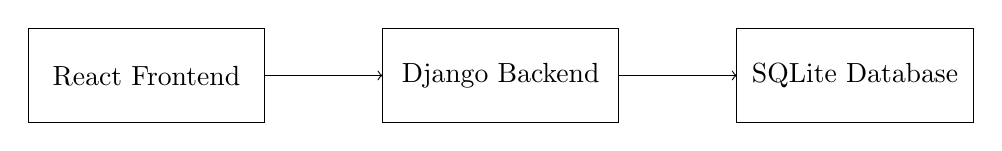
\begin{tikzpicture}
    \draw (0,0) rectangle (3,1.2);
    \node at (1.5,0.6) {React Frontend};
    \draw (4.5,0) rectangle (7.5,1.2);
    \node at (6,0.6) {Django Backend};
    \draw (9,0) rectangle (12,1.2);
    \node at (10.5,0.6) {SQLite Database};
    \draw[->] (3,0.6) -- (4.5,0.6);
    \draw[->] (7.5,0.6) -- (9,0.6);
\end{tikzpicture}
\caption{Basic architecture of the system}
\end{figure}

The frontend sends and receives data through APIs. The backend handles the
requests and communicates with the database. Administrators use Django's
built-in admin site at \texttt{/admin/}; they do not use the React website.

\subsection{How a request works}
For example, when a student presses the Enroll button:
\begin{enumerate}
    \item The browser sends a request to
    \texttt{POST /api/student/enrollments/} with the course code.
    \item The backend checks whether the request is allowed from the website.
    \item Django finds the correct view for the request.
    \item The login token is checked. If it is missing or invalid, the response
    is 401.
    \item The backend checks whether the user is a student. If the role is
    incorrect, the response is 403.
    \item The backend applies the enrollment rules and updates the database.
    \item The backend sends a response. It can indicate successful enrollment,
    a request sent for approval, invalid input or a course not found.
    \item The website displays the result and updates the course list.
\end{enumerate}

The same database is used by all users. When faculty approves an enrollment
request, the student can see the course after the page is loaded again.

\subsection{Login and user roles}
The login page sends the username, password and selected role to
\texttt{/api/auth/login/}. The backend checks the password and the selected
role. On successful login, it returns an access token, a refresh token and
the user's details. The website stores the tokens in the browser and sends the
access token with later requests. For the project demonstration, both tokens
are valid for about 100 years.

\begin{itemize}
    \item \textbf{Student:} Uses the React website and student APIs.
    \item \textbf{Faculty:} Uses the React website and faculty APIs.
    \item \textbf{Admin:} Uses the Django admin site to manage the data.
\end{itemize}

The main response codes are 200 (successful), 201 (created), 202 (request
accepted), 400 (invalid input), 401 (not logged in), 403 (access not allowed)
and 404 (not found).

\section{Database Design}

The project stores its information in 12 tables created using Django models.

\begin{itemize}
    \item \textbf{User:} Stores username, password hash and role.
    \item \textbf{Student:} Stores roll number, name, email, department and year.
    It is connected one-to-one with User.
    \item \textbf{Faculty:} Stores name, email and department. It is connected
    one-to-one with User.
    \item \textbf{Course:} Stores course code, name, credits and capacity. Each
    course is taught by one faculty member, and its code is unique.
    \item \textbf{CourseSchedule:} Stores start time, end time and room. Each
    course has one schedule. A room cannot be used twice at the same start time,
    and the end time must be after the start time.
    \item \textbf{Enrollment:} Connects a student and a course. The same student
    cannot be enrolled in the same course twice.
    \item \textbf{EnrollmentRequest:} Stores the request status and dates. A
    faculty member decides the request. Only one pending request is allowed
    for a student and course.
    \item \textbf{Assignment:} Stores title, description, due date and maximum
    marks for a course.
    \item \textbf{Submission:} Stores the submission date and connects a student
    with an assignment. Each pair is stored only once.
    \item \textbf{Grade:} Stores marks, letter grade and remarks. It is connected
    one-to-one with a submission.
    \item \textbf{PreviousCourse:} Stores the code, name and credits of an
    earlier course and the faculty member who taught it.
    \item \textbf{PreviousEnrollment:} Stores a student's grade, classes held,
    classes attended and completion status for a previous course.
\end{itemize}

A faculty member who teaches a course cannot be deleted. Deleting a student
also removes their enrollments and submissions.

\textbf{Why User and Student are separate:} Every person needs a login account,
but only students have a roll number and year. Login details are stored in User,
while student or faculty details are stored in their respective tables. Both
tables share the same user ID.

\section{Implementation}

\subsection{Backend}
The backend is divided into the following parts:
\begin{itemize}
    \item \texttt{config/}: Contains project settings and the main URL list.
    \item \texttt{accounts/}: Contains user, student and faculty models, login,
    permission checks and admin pages.
    \item \texttt{courses/}: Contains course-related models, serializers, views,
    enrollment rules, admin pages and commands to import data.
\end{itemize}

The general working order is: URL, view, permission check, database operation
and response sent as JSON.

\subsection{Main API addresses}
All API addresses except login need a valid token.

\begin{itemize}
    \item \textbf{Login:} \texttt{POST /api/auth/login/}
    \item \textbf{User details:} \texttt{GET /api/auth/me/}
    \item \textbf{Refresh token:} \texttt{POST /api/auth/refresh/}
    \item \textbf{Student courses:} \texttt{GET /api/student/courses/}
    \item \textbf{Available courses:} \texttt{GET /api/student/courses/available/}
    \item \textbf{Previous courses:} \texttt{GET /api/student/courses/previous/}
    \item \textbf{Course assignments:}\\ \texttt{GET /api/student/courses/<code>/assignments/}
    \item \textbf{Student grades:} \texttt{GET /api/student/grades/} and
    \texttt{/marks/}
    \item \textbf{Student timetable:} \texttt{GET /api/student/schedule/}
    \item \textbf{Enrollment:} \texttt{POST /api/student/enrollments/}
    \item \textbf{Faculty courses:} \texttt{GET /api/faculty/courses/}
    \item \textbf{Students in a course:}\\ \texttt{GET /api/faculty/courses/<code>/students/}
    \item \textbf{Enrollment requests:} \texttt{GET /api/faculty/enrollment-requests/}
    \item \textbf{Approve or reject:}\\ \texttt{POST .../enrollment-requests/<id>/approve/}
    or \texttt{/reject/}
    \item \textbf{Faculty timetable:} \texttt{GET /api/faculty/schedule/}
    \item \textbf{Faculty grades:}\\ \texttt{GET /api/faculty/grades/} and
    \texttt{/grades/<code>/students/}
    \item \textbf{Assignments:}\\ \texttt{GET /api/faculty/assignments/} and
    \texttt{GET, POST /api/faculty/courses/<code>/assignments/}
\end{itemize}

\subsection{Important rules}
\begin{itemize}
    \item \textbf{Enrollment:} Students can directly enroll in courses from their
    own department or in the open elective (DS). For courses from other
    departments, a request is sent to the faculty member. Available seats are
    checked both when the request is made and when it is approved. A student
    cannot have two pending requests for the same course.
    \item \textbf{Assignment status:} It is shown as submitted if a submission
    exists, pending if the due date is today or later and no submission exists,
    and missing if the due date has passed and no submission exists.
    \item \textbf{Creating assignments:} The title and due date are required.
    The title must be unique in that course, the due date cannot be in the past,
    and maximum marks must be at least 1.
    \item \textbf{Previous courses:} Attendance below 60\% gives grade DX and
    status Failed. Grade F also means Failed. Other grades mean Completed.
    \item \textbf{Course ownership:} Faculty members can view and change only
    their own courses. Another faculty member's course is not accessible to them.
\end{itemize}

\subsection{Admin site}
We used Django's built-in admin site instead of creating a separate admin page.
The administrator can add and edit users, students, faculty members, courses
and enrollments, transfer a student to another course and deactivate users.
The admin forms also check the following rules:
\begin{itemize}
    \item Course capacity cannot be less than the number of enrolled students.
    \item An enrollment or transfer cannot exceed the available seats.
    \item A student cannot be enrolled in the same course twice.
    \item A course with students and a faculty member who teaches courses cannot
    be deleted.
    \item Marks cannot be greater than the assignment's maximum marks.
    \item Grade DX is allowed only when attendance is below 60\%.
\end{itemize}

\subsection{Frontend}
The frontend uses the browser's \texttt{fetch} function to communicate with
the backend. For example, the login page sends the username, password and role
to the login API. The backend returns a response, and the website either shows
an error message or saves the tokens and opens the dashboard. Later requests
send the access token. If the backend returns 401, the website logs the user out.

The main pages are:
\begin{itemize}
    \item \textbf{Student:} Dashboard, My Courses, assignments, grades, schedule
    and announcements.
    \item \textbf{Faculty:} Dashboard, courses, students, enrollment requests,
    assignments, grades, schedule and reports.
\end{itemize}

\textbf{Screenshots:} Add screenshots of the login page, one student page, one
faculty page and the admin site here.

\section{Automation}

The Bash script \texttt{setup.sh} helps set up the project using:
\begin{verbatim}
bash setup.sh
\end{verbatim}

The script performs these steps:
\begin{enumerate}
    \item Checks whether Python 3.12 or newer and Node.js are installed.
    \item Creates the Python virtual environment.
    \item Installs the Python packages.
    \item Creates the database tables using migrations.
    \item Imports the sample data using seven commands in the correct order.
    \item Checks whether the number of rows in each table is correct.
    \item Installs the frontend packages.
\end{enumerate}

The script also has \texttt{--skip-frontend}, \texttt{--reset} and
\texttt{--help} options. The reset option rebuilds the database after asking
for confirmation. The script works on macOS, Linux and Windows with Git Bash.
The project uses a \texttt{.gitattributes} file to keep Unix line endings.
On a clean copy, setup takes about 25 seconds.

\section{Testing}

We tested login, access control and the main rules of the project. The following
are the test cases prepared for the system.

\begin{enumerate}
    \item Correct student login: expected result is 200 with token and user details.
    \item Wrong password: expected result is 400 with an error message.
    \item Student selects the Faculty tab: expected result is 400.
    \item Student opens an API without a token: expected result is 401.
    \item Student opens a faculty API: expected result is 403.
    \item Student enrolls in a course from their department: expected result is 201.
    \item Student requests a course from another department: expected result is 202.
    \item Student enrolls in the same course twice: expected result is 400.
    \item Student tries to enroll in a full course: expected result is 400.
    \item Faculty approves a request: student should be enrolled.
    \item Faculty approves a request when the course is full: request should be refused.
    \item Faculty opens another faculty member's course: expected result is 404.
    \item Assignment is created with a past due date: expected result is 400.
    \item Assignment is created with a duplicate title: expected result is 400.
    \item A new assignment should appear as pending for enrolled students.
    \item Admin reduces capacity below the enrolled student count: change should be refused.
    \item Admin tries to delete a course with students: deletion should be refused.
\end{enumerate}

The result of each test should be marked as Pass or Fail after running the test
cases again.

\section{Profiling and Performance}

We used the following tools to check the performance:
\begin{itemize}
    \item \texttt{cProfile} and \texttt{pstats} to see where Python spends time.
    \item Django's \texttt{CaptureQueriesContext} to count database queries.
    \item \texttt{time.perf\_counter} to measure response time.
    \item Lighthouse to check the performance of the website.
\end{itemize}

The profiling scripts are in the backend folder named \texttt{profiling/}.

All 15 student and faculty API endpoints take about 0.3 to 1.1 milliseconds
and use 1 to 4 database queries.

A login takes about 90 milliseconds. Most of this time is used for password
checking. Importing 163 users takes about 15.4 seconds because passwords are
hashed using 1,500,000 rounds. We kept this because password hashing helps
protect stored passwords, and the delay happens during setup.

The admin Grades page initially used 106 database queries. The same course
information was loaded repeatedly. After changing the code to load related
information together, the number of queries became 6.

The admin Faculty page initially used 18 queries to count courses. After
changing the code to do the counting together, it used 6 queries.

\begin{table}[H]
\centering
\begin{tabular}{lrr}
\toprule
\textbf{Admin page} & \textbf{Before} & \textbf{After} \\
\midrule
Grades & 106 & 6 \\
Faculty & 18 & 6 \\
\bottomrule
\end{tabular}
\end{table}

The Lighthouse score for the built login page was 100 for performance, 95 for
accessibility and 100 for best practices. The frontend build is about 330 KB
of JavaScript (100 KB compressed) and 28 KB of CSS. The Lighthouse test should
be run again after the frontend is final.

\section{Team Contributions}

The following table combines Git accounts that belong to the same team member.
The contribution details are based on the project work and Git history.

\begin{table}[H]
\centering
\begin{tabular}{p{3.0cm}p{10.5cm}}
\toprule
\textbf{Team member} & \textbf{Contribution} \\
\midrule
Premi & Backend setup, JWT login, role permissions, student and faculty
APIs, enrollment rules, admin site, query profiling and merging. \\
Shalini & Login page, student dashboard, My Courses page, React
components, routing, API calls and grades table. \\
Akshitha & Frontend dashboards, navigation, search, faculty assignment page,
Bash setup script and course table design. Git accounts combined:
SaiAkshithaK and Akshitha. \\
Ridhima Kumari & User table with hashed passwords, first student API,
LaTeX project report and Beamer presentation.
  \\
Tejaswini & Course-related models and migrations, data import commands,
student assignment, grade and schedule APIs, and students and faculty table
design. Git accounts combined: Tejaswini-C468 and Chitturi. \\
\bottomrule
\end{tabular}
\end{table}

\textbf{Note on Ridhima Kumari's commits.} Ridhima's four commits
(\texttt{416cf2c}, \texttt{3a4aa5e}, \texttt{28d0f29} and \texttt{886992d})
were made with a placeholder e-mail address in her local Git configuration.
GitHub links commits to an account through the e-mail address, so on the
repository's Contributors page these commits appear under the account
\texttt{sankalpait}, which is not a member of our team. The author name stored
in each commit is ``Ridhima'', and the commit history shows her work: the user
table with hashed passwords and the first student endpoint
(\texttt{GET /api/student/courses/}). Her own GitHub account is
\texttt{Ridhima-kumari}.

The team worked with client-server architecture, APIs, database tables and
relationships, Django models, migrations, token-based login, role checking,
data import, admin pages, performance checking, React, Bash scripting and
Git collaboration.

\section{Limitations and Future Work}

\begin{itemize}
    \item Students cannot submit assignments yet. The submissions shown come
    from sample data.
    \item Faculty members cannot edit or delete assignments or enter marks yet.
    \item Announcements are fixed text and are not connected to the backend.
    \item Login is stored for each browser address, so two different users
    cannot be logged in using two tabs of the same address.
    \item The faculty page must be reloaded to show new enrollment requests.
    \item The tokens are valid for about 100 years for the demonstration. A real
    system should use a shorter validity period.
    \item SQLite is suitable for this project size. A larger system may need a
    server database.
\end{itemize}

\section{Conclusion}

We developed a course management system with student, faculty and admin roles.
It includes a React website, a Django backend, an SQLite database, token-based
login and role-based access. The backend applies the enrollment rules, the
setup process is automated, and performance checking helped reduce the number
of database queries on two admin pages. Through this project, we learned how
the frontend, backend, APIs and database work together.

\section*{Appendix: Project Files}

\begin{itemize}
    \item Repository:
    \texttt{https://github.com/}\\\texttt{shaliniveluru00-cloud/Course-Management}
    \item Backend documentation:
    \texttt{campusmanagement-backend/README.md}
    \item Frontend documentation:
    \texttt{campusmanagement-frontend/README.md}
    \item Profiling report:
    \texttt{campusmanagement-backend/profiling/PROFILING.md}
    \item Setup script: \texttt{setup.sh}
\end{itemize}

\end{document}